%!TEX root = ../Thesis.tex
\section{Data Preparation}
% aabo2017correlation
% aabo2018integrated
% dramsch2018gaussian

In \cref{sec:dataprep} I include one published journal paper \citep{aabo2018integrated}, one published conference paper \citep{aabo2017correlation}, and one published workshop paper \citep{dramsch2018gaussian}. The published conference paper with the title \citetitle{aabo2017correlation} contains preliminary work contributing to and extended in the journal paper \citetitle{aabo2018integrated}. Whereas, the workshop paper with the title \citetitle{dramsch2018gaussian} is an independent study of backscatter scanning-electron microscopy data on chalk thin slices.

The data for this thesis was acquired in the Danish North Sea. The main hydrocarbon reservoirs in the Danish Central Graben area consist of chalk, a sedimentologically distinct feature in the seismic data. The chalk layer is high in porosity (20-35\%), however, very low in permeability 3~mD to less than 1~mD. In \citet{aabo2017correlation} we presented an integrated fracture study of the Ekofisk chalk Kraka field in the South Central Graben. Within this preliminary study, we performed a localized fracture study along one well-bore to compare fracture measurements from core, well logs and seismic data. Initial analysis of the seismic data showed a maximum vertical resolution of \~40~m, which did not yield sufficient results for comparative study. 
% These data were prepared individually by three researchers, with my contribution being the analysis and preparation of the seismic dataset. 

\begin{figure}[!ht]
    \centering
    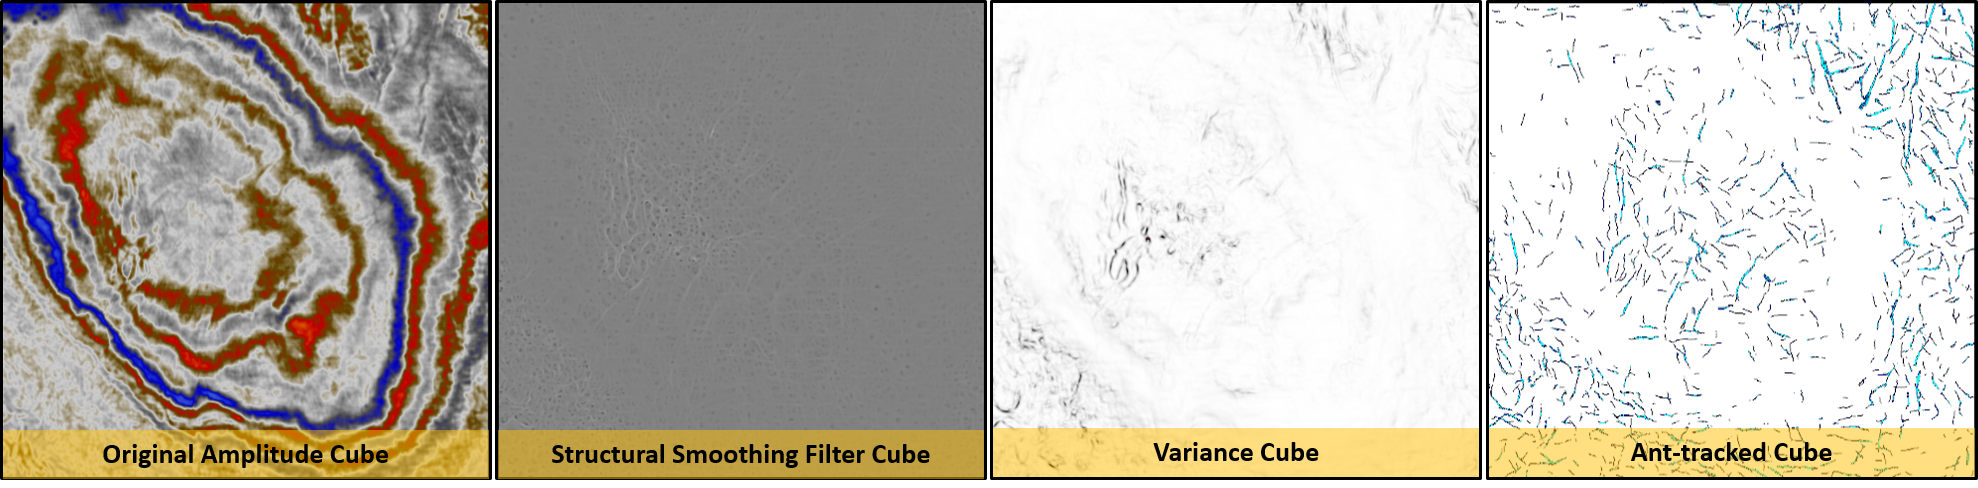
\includegraphics[width=\textwidth]{figures/seismic-comparisons.png}
    \caption{Comparison of seismic data, structural smoothed, variance and ant-track time slice \citep[modified from][]{aabo2018integrated}}
    \label{fig:seismic-comparison}
\end{figure}

\cref{fig:seismic-comparison} contains several post-stack seismic attributes to enhance lineaments within the seismic cubes. While the variance and structural cubes yielded some initial promise the following image processing workflow yielded the best results. These were geared towards enhancing vertically coherent structures. This was achieved by a workflow including colorspace transformations and ant-tracking, which is a search algorithm leveraging biologically inspired software agents.

Normally, images are shown in \ac{rgb} colorspace, however, these can be transformed into other space, such as, \ac{cmyk} and \ac{hsv}. The \ac{hsv} colorspace is commonly used in image analysis to detect edges on the gradient of the saturation values. Therefore, it serves as a good target colorspace for image processing. To achieve this, the bit-depth of seismic data has to be increased, considering that natural images displayed on modern monitors contain \~32 million colors with a bit-depth of 24~bit for color representation.
This is achieved by replicating the seismic cubes with a static timeshift to create an \ac{rgb} representation \citep{laake2014structural}. In our case a small shift below 3~ms to avoid loss of small-scale fractures and avoid smearing yielded the best results. 

Consequently, after a colorspace transformation to \ac{hsv}, the biologically inspired ant-track algorithm was applied to the saturation gradient volume. The ant-tracking algorithm implements unsupervised software-agents that search the vicinity in a 3D volume to find spatially coherent features \citep{dorigo1992optimization}. The software agents can be instructed to be more or less aggressive in their search, where I chose a moderate setting, which will enhance faults well but maintains nuance of the faults. The workflow for fault extraction is shown in \cref{fig:seismic-workflow}.

\begin{figure}[!ht]
    \centering
    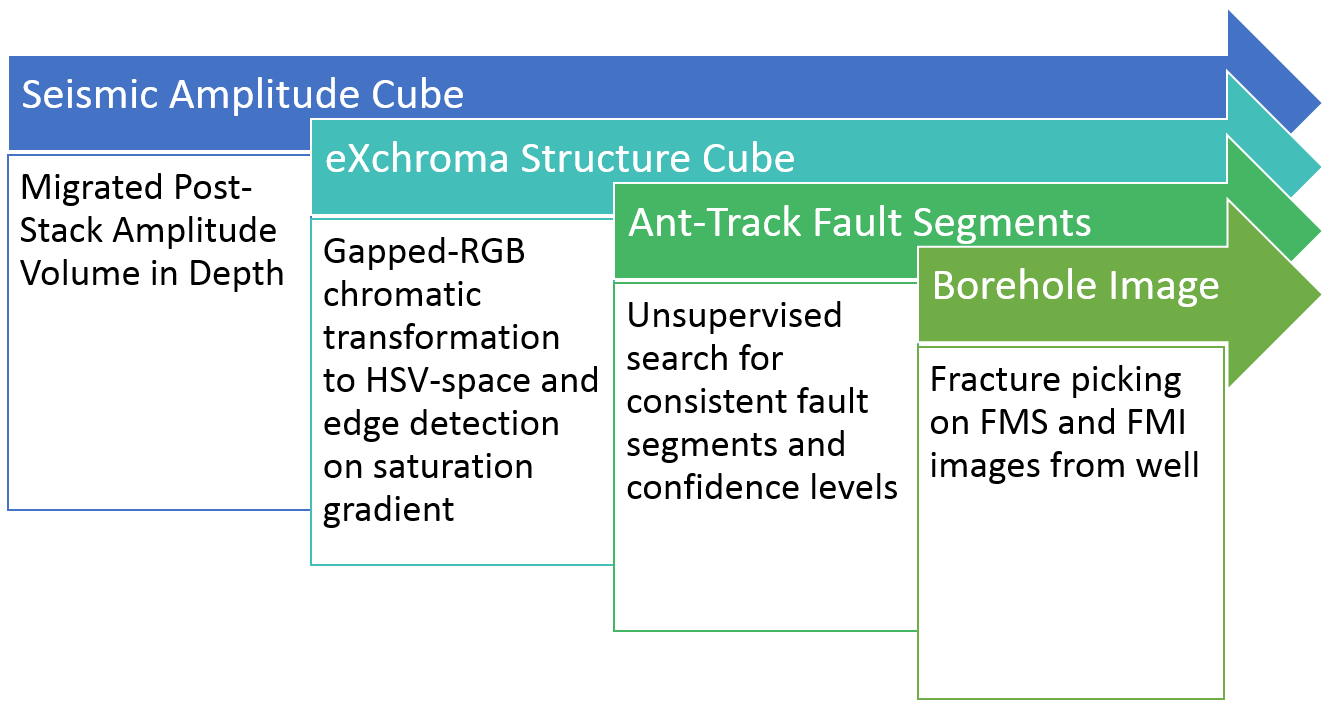
\includegraphics[width=\textwidth]{figures/fracture-workflow.PNG}
    \caption{Workflow to identify fractures in post-stack seismic data to prepare for comparison to borehole analysis}
    \label{fig:seismic-workflow}
\end{figure}

A joint interpretation of the seismic and ant-track volumes yielded a focused seismic interpretation along the well-bore, where \acf{bhi} data were available for comparison (after the interpretation to avoid bias). These match the independent interpretation of the well data closely in orientation and distribution of fractures. It is likely that these represent fracture corridors, small faults or damage zones in the chalk. This preliminary study was able to show that seismic provides a valuable method for mapping the size, orientation and connectivity of fracture zones away from the well. 

Following this initial study, the seismic interpretation was extended for to regional fault systems and \ac{bhi} to several wells for \citet{aabo2018integrated} presented in \cref{sec:tala}. The analysis of ant-tracked attribute volumes, allowed us to relate structural trends below the resolution of amplitude seismic to features at different scales. This interpretation suggests that the fracture pattern is more complex than previously suggested. We propose that fracture generation and propagation in the field is in part controlled by the regional maximum horizontal stress from the seismic interpretation in addition to the halokinesis in the South Central Graben. 

The seismic analysis was correlated with the fracture analysis from \ac{bhi} data and core analysis in multiple wells. The fracture analysis was particularly dependent on the Terzaghi-correction \citep{terzaghi1965sources} to obtain the in-situ fracture orientation. This work identified two main fracture trends in the Danian Ekofisk reservoir. The main fracture set strikes sub-parallel to the regional NE/NNE maximum horizontal stress present on all horizontal/deviated wellbores and core. The vertical fracture distribution of the Kraka Field studied in a single well, due to availability. Within this single well the NE/NNE fracture distribution was continuous. This main NNE/NE fracture trend was traced from well scale to ant-tracked scale bridgeing the scale-gap. Regional large-scale faults interpreted on the raw amplitude seismic are present in the ant-tracked cube, trending NE, which indicates that the NNE trend is representative for smaller-scale lineations, with a Northern deviation on regional scales. 

Further research into the porosity and sedimentology of the chalk reservoirs conducted on microscoping scales focused on identifying porosity using \acf{bsem} in \cref{section:gaussian}, which comprises the third paper in this chapter \citep{dramsch2018gaussian}. Identifying the grain size and orientation of the oolites is usually a manual work-intensive task, ideal for computer vision tasks, considering the good contrast of light-grey to white oolites and the black background. Unfortunately, training data was not available, which led me to experiment with unsupervised clustering to find the ideal boundary of the grain. Gaussian Mixture Models learnt a two-fold representation that separated the background well from the rock. Any single-valued decision boundary will be non-smooth, which can be alleviated by morphological filtering. Smooth boundaries are essential for chalk grains, as geologists are interested in the perimeter of the oolites to calculate the specific surface. The optimal boundary of chalk grains could then be used to generate training data for more sophisticated machine learning systems.

% This chapter enabled me to explore the Danish North Sea data in Kraka, Dan and Halfdan, as well as, implement data science principles on geological problems. Collaborating with geologists on these papers resulted in a better understanding of underlying processes in the chalk and 4D effects of production, due to compaction, stimulation and chalk weakening. The seismic analysis improved my understanding of the geological structures and trendlines in the South Central Graben area, while contributing to an improved understand of the scale-dependence of the stress fields and a method capable of extracting an optimal boundary of chalk in \ac{bsem}. 

In the first study of this chapter \citep{aabo2017correlation} I applied an image processing workflow to enhance the vertical resolution of seismic data. Consequently, I could transform the data to introduce a biologically inspired software algorithm to enhance and identify lineaments for interpretation. This work was essential in enabling a localized pilot study to relate localized features from well-scale \ac{bhi} to enhanced seismic-scale, verifying the seismic image analysis. This pilot study fed into a larger study \citep{aabo2018integrated}, where a fracture study from core and \ac{bhi} was related to both the enhanced ant-tracked volume and a regional fault interpretation, updating the understanding of the fracture generation in the Salt Dome Process in the Danish South Central Graben area. The third study solved a manual process using an unsupervised image analysis tool paired with strong data science principles, providing a novel reliable tool to geologists in \ac{bsem} analysis.